\chapter{Marco teórico}
\epigraph{\itshape Begin at the beginning, the King said gravely, <<and go on till you come to the end: then stop.>>}{---Fulano de Tal, \textit{Título del libro}}
\section{Inteligencia artificial, aprendizaje automático y aprendizaje profundo}
\todo{Reformar esta sección para incluir la IA generativa y establecer las relaciones con el resto de conceptos}
Comencemos por definir las diferentes disciplinas que intervienen en el estudio y desarrollo de sistemas de inteligencia artificial. A menudo se encuentran términos como \textit{inteligencia artificial} (\textit{Artificial Intelligence}), \textit{aprendizaje automático} (\textit{Machine Learning}) y \textit{aprendizaje profundo} (\textit{Deep Learning}) usados de forma intercambiable. Sin embargo, cada uno tiene un significado específico, y es crucial diferenciarlos para comprender el estado actual de la investigación en el área. Estos conceptos se organizan jerárquicamente \citep{torresivinalsPythonDeepLearning2020}, donde la inteligencia artificial es el término más general, que abarca el \textit{aprendizaje automático}, y este último incluye al \textit{aprendizaje profundo} (ver Figura \ref{fig:ai_ml_dl}).

\begin{figure}[H]
    \caption{Relación AI, ML y DL}
    \centering
    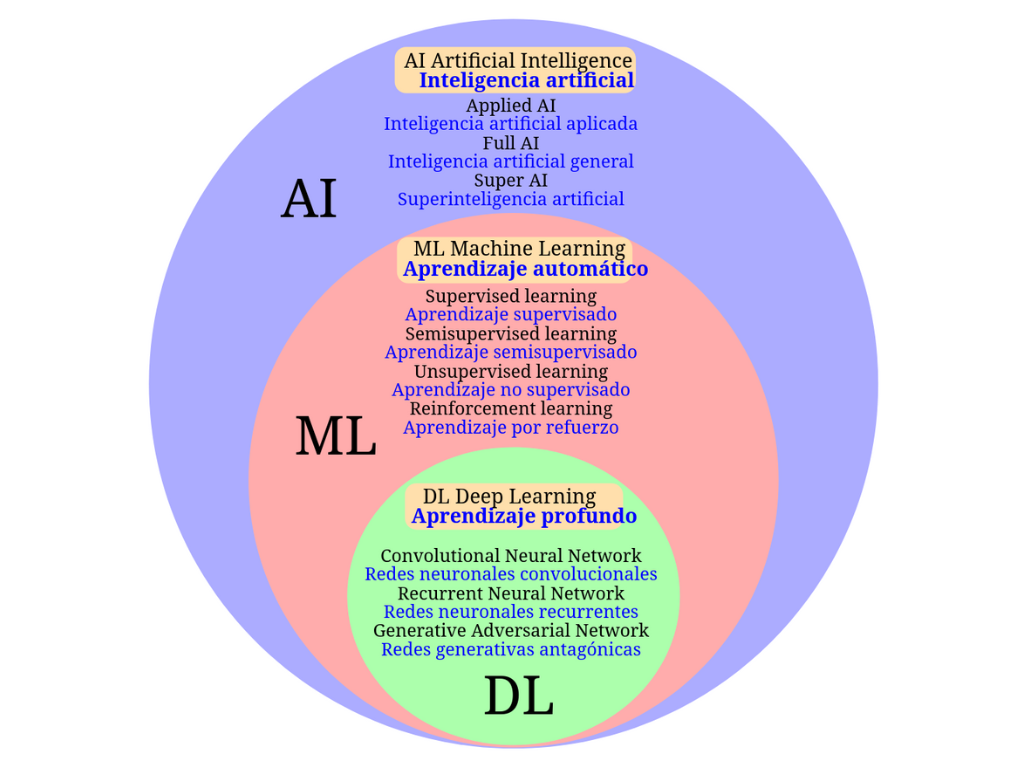
\includegraphics[width=0.8\textwidth]{./figuras/AI_ML_DL.png}
    \source{Jzh2074 \protect\citeyear{jzh2074}, Wikimedia Commons; Wang et al. \protect\citeyear{wang2021promising}.}
    \label{fig:ai_ml_dl}
\end{figure}

% He añadido una imagen de relación AI, ML, DL y AI generativa. Sería interesante modificar lo anterior para hablar también de la IA generativa, que al fin y al cabo es la que nos interesa. La imagen la he sacado de aquí: https://medium.com/@kitkat73275/introduction-to-generative-ai-833c9c467dfa (añadirla a bibliografía y citarla)


La inteligencia artificial es el campo de estudio más antiguo entre los tres, y no se limita únicamente al ámbito computacional. En su sentido más amplio, la inteligencia artificial ha sido abordada por la filosofía. Los racionalismos y estructuralismos, fundamentales en los sistemas de pensamiento occidentales, forman la base conceptual de la inteligencia artificial. Sin embargo, no es hasta el siglo XX cuando se empieza a considerar la posibilidad matemática de un sistema que genere inteligencia. En 1950, Alan Turing publicó su artículo \textit{Computing Machinery and Intelligence} \citep{alan1950a}, en el que propuso un test para determinar si una máquina puede pensar. Este test, conocido como \textit{Test de Turing}, consiste en la interacción de un humano con una entidad artificial usando solo un terminal de texto como interfaz. La máquina aprueba el test si el humano no puede discernir si está interactuando con una entidad artificial o humana. A pesar de sus limitaciones y su enfoque antropocéntrico sobre la inteligencia, este test sigue siendo una referencia común para evaluar sistemas modernos de IA.

No obstante, el concepto de inteligencia artificial trasciende la mera imitación humana, aunque no lo descarta. Si consideramos la \textit{racionalidad} como un conjunto de estructuras lógicas que incluyen el pensamiento y la racionalidad humanos, la inteligencia artificial no necesita limitar su objetivo a superar el test de Turing. Las definiciones de inteligencia artificial a lo largo del tiempo han variado dependiendo de si se enfocan en imitar el pensamiento o acción \textit{humanos} o el pensamiento y acción \textit{racional} \citep{RussellStuartJ2021AI:A}.

Debemos a matemáticos como Alan Turing y Curt Gödel los fundamentos matemáticos de los procesos de pensamiento, considerados sistemas computacionales capaces de generar \textit{outputs} racionales a partir de \textit{inputs} arbitrarios. La idea de que el cerebro humano es una de las posibles \textit{máquinas de Turing} \citep{penroseNuevaMenteEmperador2015} ha sido un estímulo para la investigación en IA computacional. Además, investigaciones en \textit{procesamiento del lenguaje natural}, en las que destaca el concepto de \textit{entropía} de Shannon \citep{shannon1951prediction} y que han acompañado el desarrollo de lenguajes de programación, son fundamentales para los sistemas actuales de IA.


\section{Machine Learning}

El \textit{Machine Learning}, o \textit{aprendizaje automático}, es una subdisciplina de la inteligencia artificial que investiga algoritmos y modelos matemáticos que habilitan a un sistema computacional a aprender a partir de datos sin ser explícitamente programado. Estos sistemas identifican patrones y toman decisiones con poca o sin intervención humana. En el \textit{Machine Learning}, el modelo se autoconfigura basándose en los datos. Las únicas intervenciones humanas son el diseño de la arquitectura y la provisión de los datos de entrenamiento, aunque incluso estas tareas podrían delegarse a otro sistema de \textit{Machine Learning} en determinadas circunstancias.

Aunque el \textit{Machine Learning} ha sido una área de interés desde los inicios de la computación, es esencial reconocer que es solo una faceta de la inteligencia artificial. No todos los sistemas inteligentes son sistemas de \textit{Machine Learning}. Por ejemplo, el \textit{Deep Blue} de IBM, que venció al campeón mundial de ajedrez Garry Kasparov en 1997, no se basaba en \textit{Machine Learning} \citep{campbellDeepBlue2002}. En lugar de ello, \textit{Deep Blue} utilizaba una vasta base de datos de jugadas de ajedrez y algoritmos de búsqueda para decidir el mejor movimiento en cada situación. Otros sistemas, como los \emph{sistemas expertos}, utilizan reglas predefinidas para tomar decisiones y se aplican en áreas como medicina, ingeniería y gestión empresarial.

En términos generales, el objetivo del \textit{Machine Learning} es encontrar una función matemática que describa un conjunto de datos de entrenamiento y que, posteriormente, pueda prever datos desconocidos con precisión. Esta capacidad predictiva se conoce como \textit{inferencia}. El proceso busca que la función determinada durante el entrenamiento aproxime la función real que describe los datos, permitiendo al sistema generalizar de forma análoga al cerebro humano.

Se utiliza el término \textit{modelo} para referirse al sistema una vez que ha sido entrenado y posee capacidad predictiva. Dependiendo de su aplicación, un modelo puede ser empleado para predecir datos desconocidos o clasificarlos. Si produce un valor numérico, se habla de \textit{regresión}; si categoriza datos, de \textit{clasificación}. La clasificación puede ser binaria o multiclase, y la regresión unidimensional o multidimensional.

El aprendizaje en \textit{Machine Learning} se produce a través de un proceso de entrenamiento. Según la naturaleza de los datos y el método de validación, existen tres tipos principales de aprendizaje automático \citep[p. ~38]{torresivinalsPythonDeepLearning2020}:

\begin{itemize}
    \item \textbf{Aprendizaje supervisado:} Aquí, los datos se etiquetan con la respuesta esperada, como imágenes de animales etiquetadas como \textit{gato} o \textit{perro}. Tras el entrenamiento, se espera que el sistema identifique imágenes no etiquetadas correctamente. Este procedimiento de aprendizaje e inferencia queda reflejado en la Figura \ref{fig:labeled_data_training}. Una de las aplicaciones más comunes del aprendizaje supervisado es la clasificación de imágenes. Sin embargo, su debilidad consiste precisamente en la necesidad de etiquetado de los datos de entrenamiento, que puede ser un proceso costoso y laborioso si este solo se puede hacer manualmente.
    
    \item \textbf{Aprendizaje no supervisado:} En este caso, los datos no están etiquetados. El sistema busca patrones y agrupa datos en categorías por sí mismo. Precisamente este es el tipo de aprendizaje utilizado en el entrenamiento de modelos de lenguaje, donde los datos de entrenamiento son textos sin etiquetar.
    
    \item \textbf{Aprendizaje por refuerzo:} El sistema aprende interactuando con un entorno. No recibe etiquetas explícitas, sino recompensas por decisiones correctas y penalizaciones por errores. Este es el modo de aprendizaje más parecido al humano, ya que se basa en la experiencia. Sin embargo, a pesar de ser uno de los métodos más atractivos de aprendizaje automático, es el más complejo de implementar y requiere un entorno de simulación adecuado, que no siempre es posible ni eficiente en términos de computación.
\end{itemize}

\begin{figure}[H]
    \caption[Esquema de aprendizaje supervisado]{Esquema de aprendizaje supervisado, usando datos de entrenamiento etiquetados. En la inferencia se espera que el modelo pueda clasificar datos no etiquetados.}
    \centering
    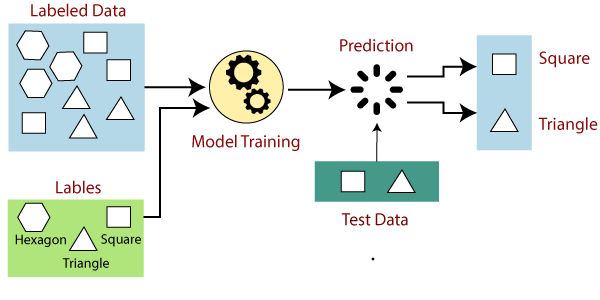
\includegraphics[width=0.4\textwidth]{./figuras/labeled_data_training.png}
    \source{\cite{FindWaysDeal}}
    \label{fig:labeled_data_training}
\end{figure}


\section{Deep Learning}

Esta sección pretende ser una somera introducción a los conceptos de \textit{Deep Learning} y \textit{redes neuronales}, que son la base de los modelos de lenguaje, objeto de nuestro estudio, con la única finalidad de aportar un aparato teórico mínimo en el que contextualizarlo. En los últimos meses la bibliografía sobre este tema ha crecido exponencialmente. Además de las obras citadas en este trabajo, se puede consultar, a modo de introducción para no especialistas, \cite{BeginnerGuideNeural}. El \textit{Deep Learning} es una subdisciplina del \textit{Machine Learning} que utiliza redes neuronales artificiales para aprender de forma automática. Las redes neuronales artificiales son modelos matemáticos que imitan el funcionamiento de las neuronas biológicas y hunden sus raíces en la intersección entre biología, matemáticas y ciencias de la computación en la primera mitad del siglo XX....

\subsection{El concepto de neurona artificial}

Para entender el funcionamiento de una red neuronal y, por extensión, de un modelo de \textit{Deep Learning}, antes es necesario comprender el de la <<neurona artificial>>. Una neurona artificial no es sino un modelo simplificado de una neurona natural que encontramos en el sistema nervioso de los animales. Análogamente a su homóloga biológica, una neurona artificial recibe una serie de entradas, las procesa y devuelve una salida. La entrada de una neurona artificial es la suma ponderada de las salidas de las neuronas de la capa anterior. Esta suma ponderada se pasa a una función de activación, que determina la salida de la neurona. Sin necesidad de entrar en detalles matemáticos, la función de activación más común es la función sigmoide, que devuelve un valor entre 0 y 1 de una forma no lineal. La Figura \ref{fig:neurona_artificial_natural} muestra un esquema de una neurona artificial. 

\begin{figure}[H]
    \caption[Neurona biológica y neurona artificial o <<perceptrón>>]{Neurona biológica y neurona artificial o <<perceptrón>>}
    \centering
    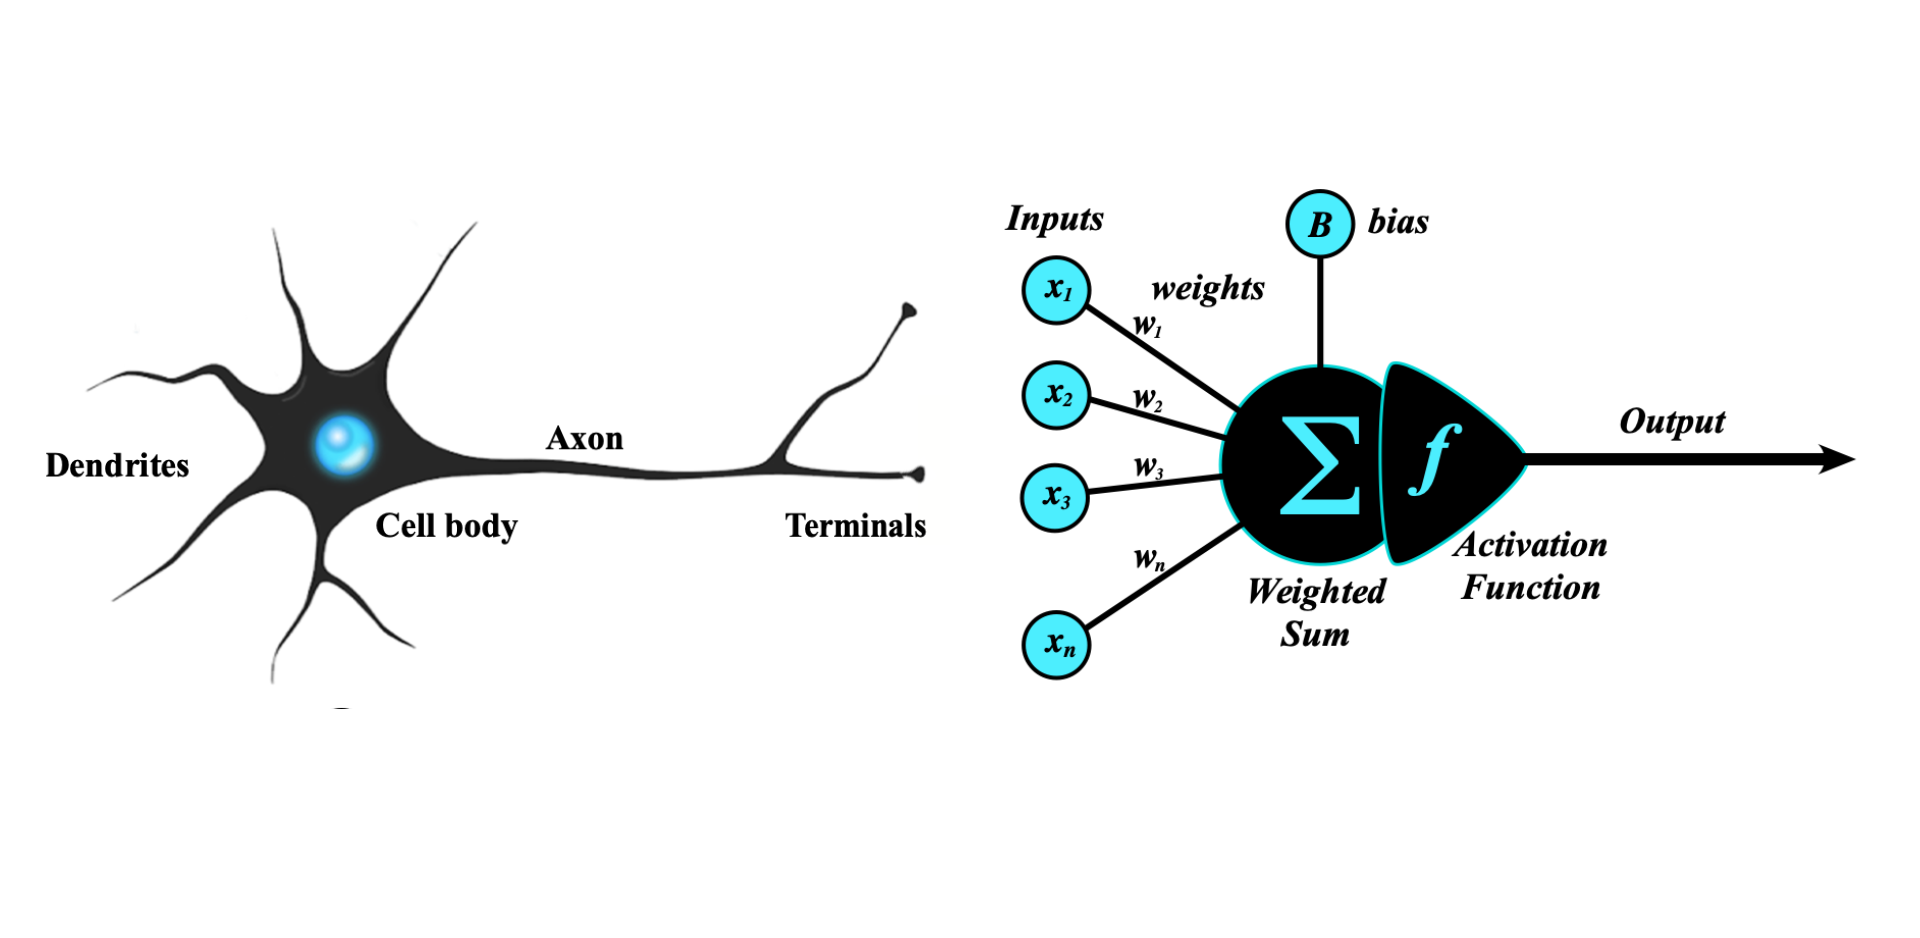
\includegraphics[width=0.4\textwidth]{./figuras/perceptron_with_neuron.png}
    \source{\cite{DeepLearningDL}}
    \label{fig:neurona_artificial_natural}
\end{figure}

Este concepto fue expuesto por primera vez por F. Rosenblatt en 1958 \citep{rothmanTransformersNaturalLanguage2021} bajo el nombre de <<perceptrón>>. El perceptrón no era otra cosa que un modelo de clasificación binaria, es decir, solo puede clasificar datos en dos categorías. Rosenblatt planteo su modelo para ser implementado en hardware, y de hecho se construyó un prototipo en 1959. Sin embargo, el perceptrón tenía limitaciones que no permitían su aplicación a problemas más complejos. Sin embargo, en 1969, Minsky y Papert publicaron un libro \citep{minsky1969perceptrons} en el que demostraban que el perceptrón no podía resolver problemas linealmente no separables. Este hecho supuso un freno en la investigación en redes neuronales artificiales, que no se retomó hasta la década de los 80, cuando se desarrollaron nuevos modelos de redes neuronales artificiales que permitían resolver problemas más complejos. Actualmente sabemos que una red neuronal de varias capas puede aproximar arbitrariamente cualquier función matemática, lo que ha venido a llamarse <<teorema de la aproximación universal>>, propuesto en 1989 por Hornik en su artículo \textit{Multilayer feedforward networks are universal approximators} \citep{hornikMultilayerFeedforwardNetworks1989}. Este teorema tiene grandes implicaciones no solo científicas, sino también filosóficas, en la medida en que podemos considerar que una red neuronal artificial es capaz de imitar el funcionamiento del cerebro humano y su comportamiento, el cual puede reducirse al de una función matemática, por compleja que esta sea, o a la ya citada <<máquina de Turing>> \citep{penroseNuevaMenteEmperador2015}.


\subsection{Redes neuronales artificiales}
Precisamente el teorema de la aproximación universal emerge de la combinación de varias capas de neuronas artificiales. Una red neuronal artificial es un modelo matemático que se compone de varias capas de neuronas artificiales. La primera capa se denomina <<capa de entrada>> y recibe los datos de entrada. La última capa se denomina <<capa de salida>> y devuelve la predicción del modelo. Las capas intermedias se denominan <<capas ocultas>> y son las que permiten que el modelo pueda aproximar cualquier función matemática. La Figura \ref{fig:deep_neural_network} muestra un esquema de una red neuronal artificial con una capa de entrada, dos capas ocultas y una capa de salida.

La salida de la neurona se pasa a las neuronas de la capa siguiente, y así sucesivamente hasta llegar a la capa de salida. La salida de esta última capa es la predicción del modelo. 

\begin{figure}[H]
    \caption[Estructura de capas de una red neuronal artificial]{Estructura de capas de una red neuronal artificial, con una capa de entrada, dos capas ocultas y una capa de salida.}
    \centering
    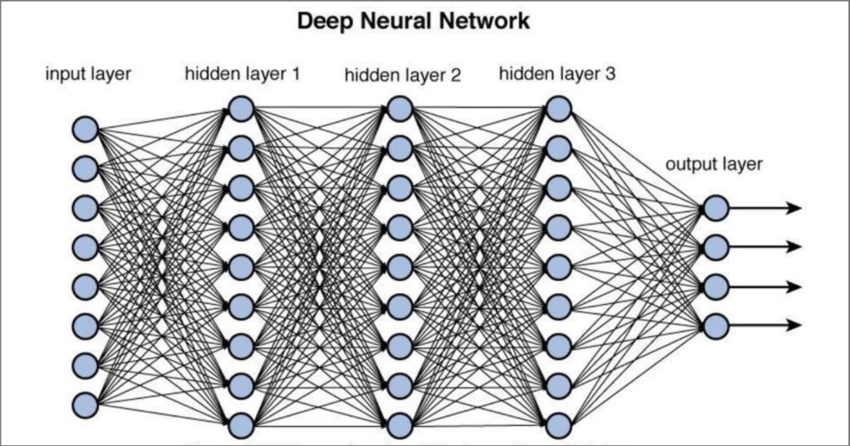
\includegraphics[width=0.4\textwidth]{./figuras/Deep_neural_network.png}
    \source{\cite{zraraPORTFOLIOOPTIMIZATIONUSING2021}}
    \label{fig:deep_neural_network}
\end{figure}

En función de los objetivos de la red neuronal, la arquectura, o estructura interna, puede variar considerablemente. Una red neuronal puede constar de una sola capa, de una capa de entrada y otra de salida, y de múltiples capas ocultas. Cada arquitectura busca resolver un tipo de problema concreto. Una arquitectura especialmente compleja, y que ha dado muy buenos resultados en la visión artificial es la red convolucional, inspirada en el funcionamiento de la corteza visual del cerebro humano. Las redes convolucionales se utilizan para el reconocimiento de imágenes y vídeos, y han sido la base de los avances en el campo de la visión artificial en los últimos años.

Independientemente de su estructura, una red neuronal o modelo de \textit{Deep Learning} debe ser entrenado para que pueda aprender a partir de los datos. El proceso de entrenamiento consiste en presentar los datos de entrenamiento a la red neuronal y ajustar los parámetros internos de la red para que la salida se aproxime a la salida esperada. Este proceso se repite iterativamente hasta que la salida de la red neuronal se aproxima a la salida esperada con un margen de error aceptable. Una vez entrenada, la red neuronal puede predecir la salida de datos desconocidos. Este proceso se ilustra en la Figura ... Por parámetros internos entendemos los pesos de las conexiones entre neuronas, que son los que en definitiva determinan la salida de la red neuronal. Un modelo antes de ser entrenado da como salida valores aleatorios, y el entreamiento consiste en ajustar estos valores para que la salida se aproxime a lo esperado. Existe una relación, grosso modo, entre la cantidad de parámetros (pesos) de un modelo y su capacidad predictiva, al tiempo que aumenta considerablemente el tiempo de entrenamiento y la capacidad computacional necesaria para entrenarlo. Esta es una de las razones por las que ha habido que esperar a los últimos años para empezar a ver resultados equiparables a los del cerebro humano, especialmente en tareas de generación de imágenes, vídeo, audio o texto.

\subsection{La arquitectura Transformer}
Hasta 2017, el estado del arte en el ámbito del procesamiento de lenguaje natural por medio de modelos de \textit{Deep Learning} eran las redes neuronales recurrentes (RNN). Estas se basaban en la idea de que la salida de una neurona se podía retroalimentar a la entrada, de forma que la salida de la neurona en el instante $t$ se podía usar como entrada en el instante $t+1$. Esta arquitectura se ilustra en la Figura.... Sin embargo, las RNN presentaban un problema conocido como \textit{vanishing gradient}, que hacía que el modelo no pudiera aprender de secuencias largas. Este problema se solucionó con las redes neuronales de memoria a corto y largo plazo (LSTM), que permitían que la información fluyera a través de la red sin perderse. Sin embargo, las LSTM no podían trabajar con grandes cantidades de tokens de contexto, lo que limitaba su aplicación a tareas de procesamiento de lenguaje natural.

Sin embargo, en 2017, \citeauthor{vaswaniAttentionAllYou2017} publicaron un artículo \citep{vaswaniAttentionAllYou2017} en el que proponían una nueva arquitectura de red neuronal, denominada \textit{Transformer}, que no se basaba en las RNN y que permitía trabajar con grandes cantidades de tokens de contexto. Esta arquitectura se basaba en el concepto de \textit{atención}, que permite que el modelo pueda aprender de secuencias largas. En esta arquitectura, no importa la posición de los tokens de la secuencia de entrada, ya que el modelo aprende a asignar pesos a cada token en función de su relevancia para la predicción del siguiente token. A diferencia de una RNN, un \textit{Transformer} puede procesar todos los tokens de una secuencia de entrada en paralelo, lo que lo hace mucho más eficiente computacionalmente tanto en el entrenamiento como en la inferencia. La Figura \ref{fig:transformer_attention} muestra una matriz de atención de un \textit{Transformer} entrenado con textos en inglés.

En la figura \ref{fig:transformer_architecture} se puede ver un esquema de la arquitectura \textit{Transformer}.

\begin{figure}[H]
    \caption[Aquitectura de Transformer]{Aquitectura de Transformer}
    \centering
    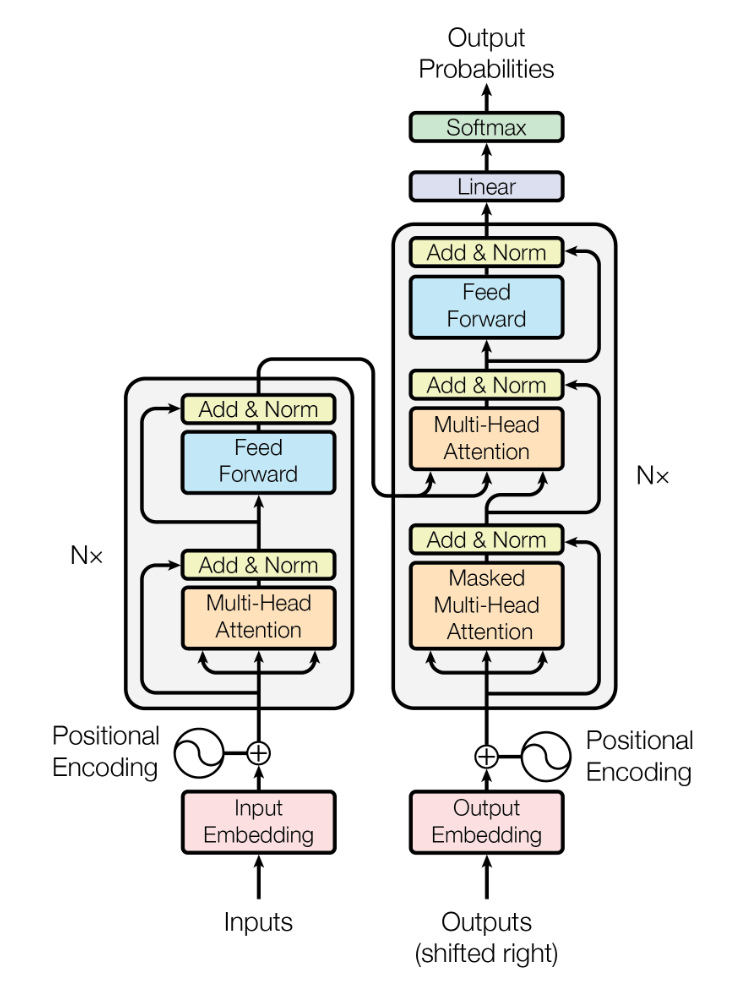
\includegraphics[width=0.4\textwidth]{./figuras/Transformer_architecture.png}
    \source{\cite{vaswaniAttentionAllYou2017}}
    \label{fig:transformer_architecture}
\end{figure}

\begin{figure}[H]
    \caption[Matriz de \textit{atención} de un \textit{Transformer} entrenado con textos en inglés]{Matriz de \textit{atención} de un \textit{Transformer} entrenado con textos en inglés. En ella queda representada la atención de cada token de la secuencia de entrada <<He later went to report Malaysia for one year>> con respecto a los demás.}
    \centering
    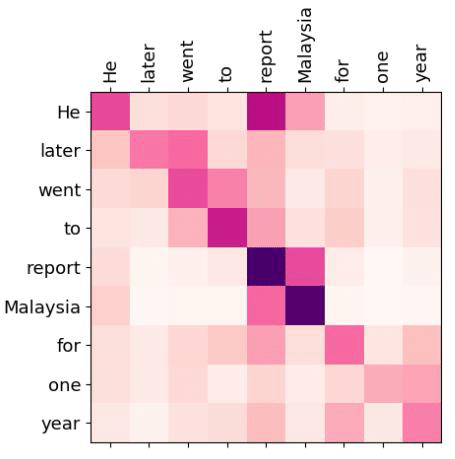
\includegraphics[width=0.4\textwidth]{./figuras/Transformer_attention_matrix.png}
    \source{\cite{duAddressingSyntaxBasedSemantic2022}}
    \label{fig:transformer_attention}
\end{figure}

\section{Modelos de lenguaje}

Un \textit{modelo de lenguaje} es un modelo estadístico que asigna una probabilidad a una secuencia de palabras dada como entrada. Esencialmente, es una función matemática diseñada para simular la forma en que se escribe en lenguaje natural. Una analogía común para entender el funcionamiento de un \textit{modelo de lenguaje} es la función predictiva de un teclado. Mientras escribimos en nuestro dispositivo móvil, el teclado nos sugiere palabras que probablemente seguirán a las ingresadas. Esta capacidad de predicción es el fundamento de los \textit{modelos de lenguaje}, incluyendo chatbots avanzados.

Desde una perspectiva técnica, un \textit{modelo de lenguaje} devuelve como salida la distribución de probabilidad del siguiente \textit{token}, dada una secuencia de \textit{tokens} como entrada \citep{GenerationLLMs}. Un \textit{token} es la unidad mínima de información que el modelo procesa y, generalmente, equivale a una palabra\footnote{Aunque un token suele ser una palabra, también puede ser un signo de puntuación, número o cualquier otra unidad mínima de información.}. La Figura \ref{fig:llm_generation} ilustra un \textit{modelo de lenguaje} que recibe una secuencia de palabras y devuelve la distribución de probabilidad del siguiente \textit{token} después de haber sido entrenado con textos en inglés.

\begin{figure}[H]
    \caption[Inferencia de \textit{token} de un LLM]{Inferencia de \textit{token} de un LLM}
    \centering
    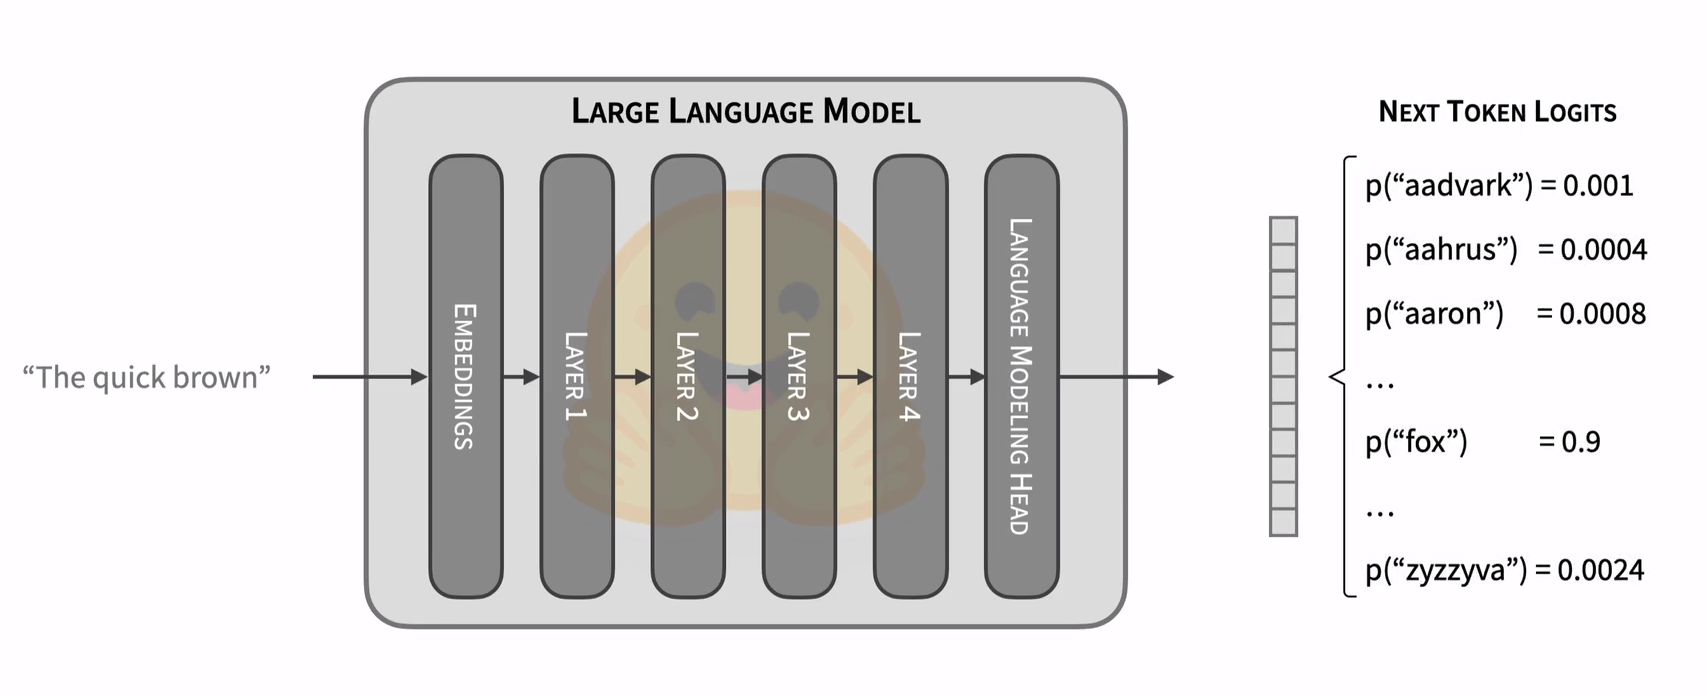
\includegraphics[width=0.9\textwidth]{./figuras/LLM_predice_token.png}
    \source{\cite{GenerationLLMs}}
    \label{fig:llm_generation}
\end{figure}

Los \textit{modelos de lenguaje} no se asocian exclusivamente a una arquitectura de \textit{Machine Learning}. Pueden implementarse mediante diferentes tipos de redes neuronales, como las redes neuronales recurrentes o convolucionales. No obstante, el hito que ha propulsado avances significativos en \textit{Machine Learning} ha sido la arquitectura \textit{Transformer} \citep{vaswaniAttentionAllYou2017}, de la que se ha hablado más arriba.

\subsection{Grandes modelos de lenguaje}

Un \textit{gran modelo de lenguaje} (LLM) posee un número de parámetros del orden del billón, lo cual es considerado <<grande>> o \textit{large} desde el punto de vista computacional. El primer LLM fue \textit{GPT-2}, creado y entrenado por OpenAI en 2019 \citep{radfordLanguageModelsAre2019a}. \textit{GPT-2} se entrenó con 40 GB de texto de Internet y alcanzó 1.5 billones de parámetros. Su capacidad para predecir la siguiente palabra en una secuencia sorprendió a la comunidad científica debido a la calidad de los textos generados. Sin embargo, OpenAI publicó una versión reducida de 117 millones de parámetros debido a preocupaciones sobre su eventual uso irresponsable. La Figura \ref{fig:gpt2_text_generation} muestra ejemplos de textos generados por este modelo.

\begin{figure}[H]
    \caption{Generación de textos por \textit{GPT-2}}
    \centering
    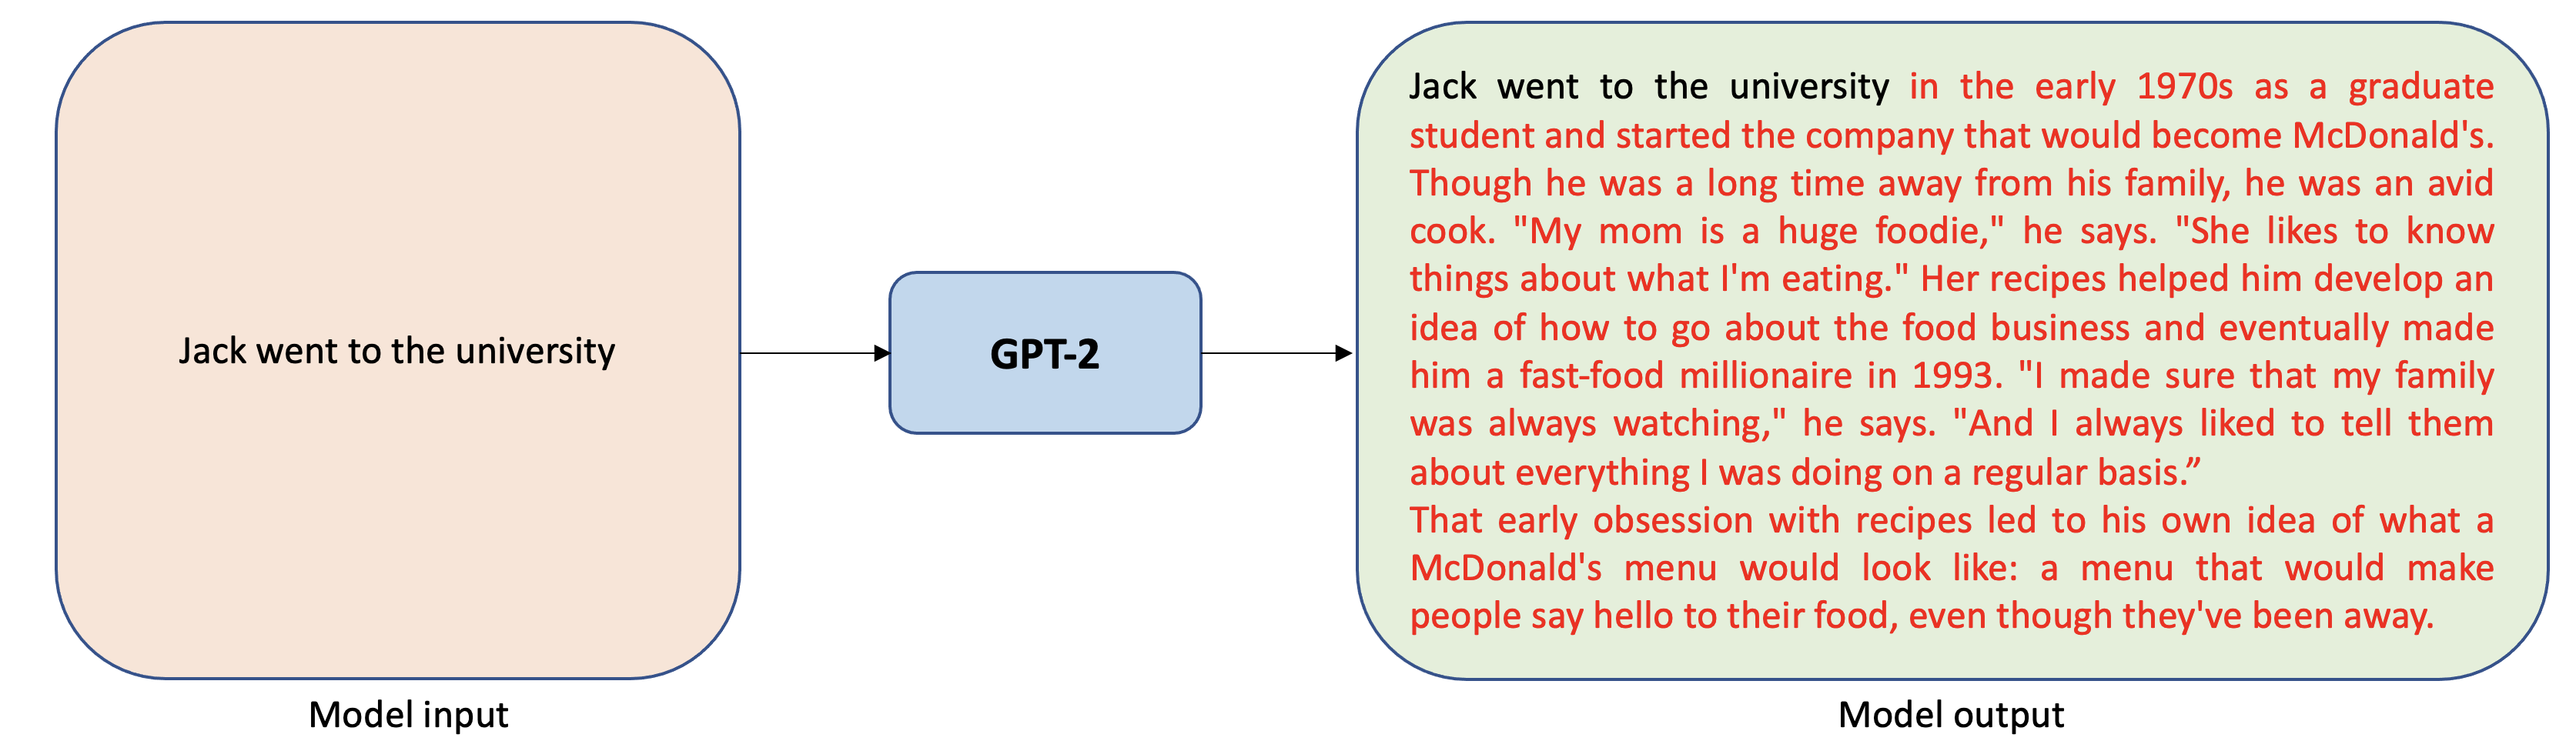
\includegraphics[width=0.9\textwidth]{./figuras/GPT2_text_generation.png}
    \source{\cite{RunTextGeneration2022}}
    \label{fig:gpt2_text_generation}
\end{figure}

Los \textit{grandes modelos de lenguaje} emplean la arquitectura \textit{Transformer} o derivados. Se entrenan con grandes cantidades de texto sin etiquetar, como libros, artículos de periódicos, páginas web, etc., realizándose este proceso en paralelo, lo que requiere una gran capacidad computacional. Sin embargo, una vez entrenados, estos modelos pueden ser utilizados para tareas de generación de texto, traducción automática, resumen de textos, etc. con una capacidad predictiva sorprendente. La Figura \ref{fig:llm_sizes} muestra una comparativa de los tamaños de los LLM más conocidos.

\begin{figure}[H]
    \caption{Gráfico comparativo de tamaños de LLM}
    \centering
    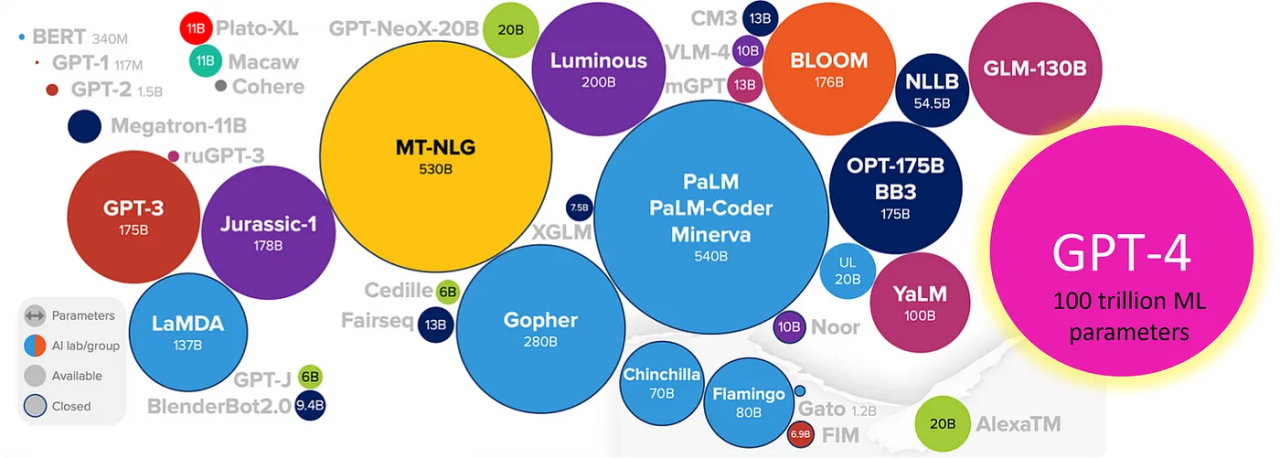
\includegraphics[width=0.9\textwidth]{./figuras/LLMs_sizes.png}
    \source{\cite{ChallengesAssociatedBuilding}}
    \label{fig:llm_sizes}
\end{figure}

\subsection{Modelos preentrenados}
\subsection{Ajuste fino de los modelos}
Bibliografía: \cite{chamandFinetuneYourClassifier2022}

\subsection{Hiperparámetros fijos del modelo}
Aquí hablaré de los hiperparámetros que definen la arquitectura del modelo que no se pueden modificar, como el número de capas, el número de cabezas de atención, etc., y que son fijos en el modelo. Especial atención se pondrá en el número de parámetros del modelo, que es el que determina el tamaño del modelo y su capacidad de generar textos, así como en la ventana de contexto, que es el número de tokens que el modelo tiene en cuenta para generar el siguiente token.

Precisamente el número de parámetros y la ventana de contexto son los hiperparámetros más importantes y críticos en términos computacionales y de efectividad. Cuanto más grande sea el modelo, más parámetros tendrá y más capacidad de generar textos tendrá. Sin embargo, también será más lento en la inferencia. Por otro lado, cuanto mayor sea la ventana de contexto, más tokens tendrá en cuenta el modelo para generar el siguiente token, y más coherentes serán los textos generados. Sin embargo, también será más lento en la inferencia.

Consideraciones interesantes sobre parámetros y ventana de contexto en \cite{gonzaloAsomandonosVentanaContextual2023}

\subsection{Hiperparámetros controlables por el usuario}
\label{sec:hiperparametros_controlables}
Hablar de la temperatura, top\_p, top\_k, ventana de contexto, número de tokens, etc. 

Se habla de la temperatura y su impacto en la generación de textos en \cite{holtzmanCuriousCaseNeural2020} y \cite{chamandFinetuneYourClassifier2022}

\cite{holtzmanCuriousCaseNeural2020} habla de la importancia de top\_p, en lo que denomina \textit{top\_k nucleus sampling}. Aunque es antiguo el paper, echar un ojo porque aclara bastante los conceptos.

Seguimos las explicaciones de \cite{rothmanTransformersNaturalLanguage2021}

Existen estudios centrados en la optimización de los hiperparámetros (los ya citados más arriba y \cite{wangCostEffectiveHyperparameterOptimization2023} y \cite{wangHyperparameterOptimizationAlgorithm2022})


\subsection{Habilidades emergentes de los modelos de lenguaje}
\subsection{Técnicas de \textit{prompting}}
\label{sec:llm_tecnicas_prompting}
En esta sección se abordará la disciplina del \textit{prompting engineering} y se ofrecerá una visión general de sus enfoques \citep{LLMPromptingGuide}\dots


\section{Limitaciones conocidas de los LLM}
Ventana de contexto, sesgos, alucinaciones, dar la razón al usuario, 










